% Provenance (never printed): see sources/outline_sources.md (Year 2: climate archives and proxies;
% foraminiferal and ice isotopes; Mg/Ca; pollen; speleothems; tree rings; dating the archives).
% Calibrations after Miller et al. (2020), Groeneveld et al. (2019) and Morley et al. (2024); ice
% cores after White (Geochemistry, ch. 9), Werner et al. (2018) and the EPICA Dome C file of Jouzel
% et al. (2007); age model after Svensson et al. (2008); deep-water context after Wharton et al.
% (2026); figures from figdata/bachelor-2/proxies.py (data/derived lr04, edc-temperature,
% co2-icecore); values of the exercises and problem computed in the Book 4 scratch calculator
% calc/ch24.py.
\chapter{Klimaatarchieven en proxy's}\label{ch:b2:climate-proxies}

In een artikel uit 1955 rapporteerde een jonge geochemicus de zuurstofisotopen van de minuscule schaaltjes van
foraminiferen, uitgezocht uit kernen van de oceaanbodem, en vond daarin vijftien glaciaal--interglaciale cycli over de
laatste \num{600000} jaar. Hij las ze vooral als temperatuur: hij schreef slechts ongeveer een vijfde van
de schommelingen toe aan het ijs dat op het land was opgeslagen. Achttien jaar later kwamen Shackleton en Opdyke tot het
omgekeerde: het belangrijkste effect was de opslag van isotopisch licht water in de
ijskappen. Dezelfde schaaltjes, dezelfde getallen, twee lezingen. Een schaal van calciet legt de
temperatuur vast van het water waarin ze groeide en de samenstelling van dat water, en de samenstelling van
zeewater hangt af van hoeveel ijs er op het land ligt. Dit hoofdstuk gaat over zulke registraties, de
archieven die ze bewaren, de proxy's die eruit worden afgelezen, hoe ze tegen thermometers worden gekalibreerd
en hoe ze worden gedateerd, en over de kunst om twee signalen te scheiden die door één schaal worden gedragen.
% ledger: white13c9:paleo-history

\begin{recall}
\textbf{Uit de schoolboeken}: \omterm{def:b2:climate-proxies:proxy}{klimaatarchief} en proxy, ijskern, glaciaal en
interglaciaal, het Laatste Glaciale Maximum (ongeveer \num{23000} tot \num{19000} jaar geleden),
pollenanalyse. \textbf{Uit Boek~3}: radiometrische datering, de radiokoolstofouderdom en zijn
kalibratiecurve; kalkslib, opgebouwd uit coccolieten en de schaaltjes van foraminiferen.
\textbf{Uit \cref{ch:b2:isotope-geochemistry}}: de \omterm{def:b2:isotope-geochemistry:standards}{isotopische referentiestandaarden} \omterm{def:b2:isotope-geochemistry:standards}{VSMOW} en \omterm{def:b2:isotope-geochemistry:standards}{VPDB}
(\cref{def:b2:isotope-geochemistry:standards}) en de \omterm{prop:b2:isotope-geochemistry:mwl}{meteorische waterlijn}, $\delta\mathrm{D}
\approx 8\,\delta^{18}\mathrm{O} + 10$ (\cref{prop:b2:isotope-geochemistry:mwl}). \textbf{Uit de
scheikundeboeken}: de $\delta$-waarde en de fractioneringsfactor. \textbf{Uit de
wiskundeboeken}: de kleinstekwadratenlijn.
\end{recall}
% ledger: ipcc:lgm-cooling, kc98:mwl, kc98:standards

\section{Archieven en proxy's}\label{sec:b2:climate-proxies:archives}

Instrumenten meten het klimaat pas sinds kort. Alles daarvoor wordt afgelezen uit materialen
die laag voor laag groeiden of bezonken terwijl het klimaat erop inwerkte: sneeuw die op de
poolijskappen tot ijs wordt, schaaltjes die op de oceaanbodem neerregenen, de jaarringen van bomen, koralen, de afzettingen van
grotten, het slib van meren. De schoolboeken noemden ze archieven en de grootheden die erin worden gemeten
proxy's; we hebben nu scherpere woorden nodig.

\begin{definition}[Klimaatarchief; klimaatproxy]\label{def:b2:climate-proxies:proxy}
Een \emph{klimaatarchief}\index{klimaatarchief} is een natuurlijk materiaal dat zich
geleidelijk ophoopt, laag op laag of ring op ring, en fysische, chemische of biologische
kenmerken bewaart van het milieu waarin elk deel ontstond. Een
\emph{klimaatproxy}\index{klimaatproxy} is een grootheid die in een archief wordt gemeten en die van een
klimaatvariabele afhangt, zoals een temperatuur, een hoeveelheid regen of een ijsvolume, via een betrekking die kan
worden gekalibreerd, en die zo de plaats inneemt van een meting van die variabele die nooit werd gedaan.
\end{definition}
% ledger: ncei:proxy, ncei:paleocean

Drie eigenschappen bepalen wat een archief kan vertellen: zijn resolutie (de tijdspanne die één
monster beslaat), zijn bereik (hoe ver het teruggaat) en hoe het wordt gedateerd. Een archief met jaarlagen kan
jaar voor jaar worden gelezen en door tellen worden gedateerd; de andere hebben radiometrische ouderdommen of vergelijking met een
gedateerde reeks nodig. De tabel hieronder vergelijkt de archieven van dit hoofdstuk.

\begin{center}
\small
\begin{tabular}{>{\raggedright\arraybackslash}p{0.17\linewidth}>{\raggedright\arraybackslash}p{0.27\linewidth}>{\raggedright\arraybackslash}p{0.21\linewidth}>{\raggedright\arraybackslash}p{0.24\linewidth}}
\hline
archief & proxy's in dit hoofdstuk & jaarlagen & datering \\
\hline
diepzeesediment & $\delta^{18}$O en Mg/Ca van foraminiferen & nee & radiokoolstof, vergelijking met
gedateerde reeksen \\
poolijs & $\delta$D en $\delta^{18}$O van het ijs, lucht in bellen & in het bovenste deel van dikke
kernen & tellen van lagen, gedateerde vulkanische lagen \\
jaarringen & ringbreedte, houtdichtheid, isotopen & ja & tellen en kruisdateren van ringen \\
\omterm{def:b2:climate-proxies:archives}{speleothemen} & $\delta^{18}$O & in sommige & radiometrische datering \\
meersedimenten & \omterm{def:b2:climate-proxies:archives}{varven}, pollen & waar gevarveerd & tellen van \omterm{def:b2:climate-proxies:archives}{varven} \\
\hline
\end{tabular}
\end{center}
% ledger: ncei:proxy, ncei:paleocean, ncei:tree-ring, ncei:speleothem, mccarthy23:varves, svensson08:gicc05, noaa:gisp2-layers, bebchuk26:crossdating

Een proxy is nooit een zuivere maat voor één variabele. De breedte van een jaarring hangt af van de warmte van
de zomer en van de regen; de $\delta^{18}$O van een schaal van de temperatuur van het water en van
zijn isotopische samenstelling. Het werk van de paleoklimatoloog is een proxy te vinden waarvan de afhankelijkheid
van de gezochte variabele sterk en bekend is, de andere invloeden onafhankelijk te meten, en het
monster te dateren.

\section{Zuurstofisotopen in kalkschalen}\label{sec:b2:climate-proxies:oxygen}

Foraminiferen zijn eencellige protisten, waarvan er veel een schaal van calciet bouwen; de planktonische
soorten zweven in het oppervlaktewater, de benthische leven op of in het sediment van de
zeebodem. Hun schalen hopen zich op in de kalkslibben van Boek~3, en de
$\delta^{18}$O van het calciet kan worden gemeten aan enkele schaaltjes die uit elke centimeter van een
kern zijn uitgezocht.
% ledger: ucmp:forams, ncei:paleocean

\begin{history}[Twee lezingen van één reeks]
Urey berekende in 1947 hoe de fractionering van zuurstof tussen calciet en water van de
temperatuur afhangt, en stelde voor dat carbonaten de temperatuur waarbij ze ontstonden, konden vastleggen. Cesare
Emiliani, toen zijn student, mat $\delta^{18}$O in foraminiferen uit zuigerkernen van de
oceanen van de wereld en publiceerde in 1955 een reeks met 15 glaciaal--interglaciale cycli over
\num{600000} jaar, waarbij hij ongeveer \qty{20}{\percent} van de variatie aan het ijsvolume toeschreef.
In 1973 concludeerden Shackleton en Opdyke dat de opslag van isotopisch licht water in de
ijskappen het belangrijkste effect was. De vitale effecten, de afwijkingen van een soort van het evenwicht,
en de uitwisseling van zuurstof met poriewater na de begraving zijn meestal niet erg belangrijk voor de
schalen van de laatste paar miljoen jaar; de isotopische samenstelling van het water wel.
\end{history}
% ledger: white13c9:paleo-history

\subsection*{Temperatuur}

Calciet dat in evenwicht met water groeit, is rijker aan \textsuperscript{18}O dan het water,
en hoe kouder het water, hoe groter de verrijking, zoals Urey's berekening liet zien. Verscheidene
empirische kalibraties verbinden
de temperatuur met het verschil tussen de $\delta^{18}$O van het calciet, op de VPDB-schaal, en
die van het water, op de VSMOW-schaal. Voor de diepzee wordt voor benthische
schalen een vereenvoudigde vorm gebruikt.

\begin{proposition}[Een benthische kalibratie]\label{prop:b2:climate-proxies:benthic}
Voor benthische foraminiferen bij diepzeetemperaturen (onder ongeveer \qty{13}{\celsius}) geldt
\[
  T = 16.1 - 4.76\,\bigl[\delta^{18}\mathrm{O}_{\mathrm{b}} - (\delta^{18}\mathrm{O}_{\mathrm{sw}} -
  0.27)\bigr],
\]
met $T$ in \unit{\celsius}, $\delta^{18}\mathrm{O}_{\mathrm{b}}$ de waarde van de schaal (promille,
\omterm{def:b2:isotope-geochemistry:standards}{VPDB}) en $\delta^{18}\mathrm{O}_{\mathrm{sw}}$ die van het zeewater (promille, \omterm{def:b2:isotope-geochemistry:standards}{VSMOW}); de term
0.27 zet het water om naar de schaal van het calciet. Een afkoeling van \qty{1}{\celsius} bij constante
samenstelling van het water verhoogt $\delta^{18}\mathrm{O}_{\mathrm{b}}$ met $1/4.76 = 0.21$ promille.
\end{proposition}
\admitted
% ledger: miller20:paleotemp, groeneveld19:anand

De vollediger vergelijking waaruit ze is vereenvoudigd, bevat een kleine kwadratische term,
$T = 16.1 - 4.64x + 0.09x^2$ met $x$ het verschil van de twee $\delta$-waarden; planktonische schalen
hebben hun eigen kalibraties, van dezelfde vorm, zoals $T = 14.9 - 4.8\,[\delta^{18}\mathrm{O} -
(\delta^{18}\mathrm{O}_{\mathrm{sw}} - 0.27)]$. Ze delen allemaal één moeilijkheid: de schaal geeft één
getal, $\delta^{18}\mathrm{O}_{\mathrm{b}}$, en de vergelijking heeft twee onbekenden, $T$ en
$\delta^{18}\mathrm{O}_{\mathrm{sw}}$. Er is een tweede, onafhankelijke proxy nodig om ze te scheiden.
% ledger: miller20:paleotemp, groeneveld19:anand

\subsection*{Het ijsvolume-effect}

Water dat uit de zee verdampt, bevat minder \textsuperscript{18}O dan de zee; terwijl de damp
poolwaarts reist en als regen of sneeuw uitvalt, raakt hij verder verarmd, en de sneeuw die de
ijskappen opbouwt, behoort tot het lichtste water op de planeet: Groenlands ijs heeft een $\delta^{18}$O van $-30$ tot $-35$
promille, Antarctisch ijs tot $-50$. Wanneer ijskappen groeien, wordt de lichte isotoop op het land opgesloten
en wordt de achtergebleven oceaan zwaarder.
% ledger: nasaeo:o18, white:d18o

\begin{definition}[IJsvolume-effect]\label{def:b2:climate-proxies:ice-volume}
Het \emph{ijsvolume-effect}\index{ijsvolume-effect} is de verandering van de
zuurstofisotopensamenstelling van de hele oceaan, veroorzaakt door de groei of het afsmelten van de continentale ijskappen, die
water opslaan dat verarmd is aan \textsuperscript{18}O; het verschuift de $\delta^{18}$O van elk carbonaat
dat in de zee ontstaat met hetzelfde bedrag, wat de temperatuur ook is.
\end{definition}
% ledger: nasaeo:o18, white13c9:ice-volume, miller20:paleotemp

\begin{omfigure}
\centering
\begin{tikzpicture}[font=\scriptsize, >=Stealth]
\foreach \col/\title in {0/{a\enspace vandaag}, 7.0/{b\enspace een glaciaal maximum}} {
  \begin{scope}[shift={(\col,0)}]
  \node[anchor=south west] at (0,3.3) {\textbf{\title}};
  \fill[brown!30] (3.6,0) -- (6.4,0) -- (6.4,1.6) -- (3.6,1.2) -- cycle;
  \end{scope}
}
% today: full ocean, small ice sheet
\fill[ocBlue!25] (0,0) rectangle (3.6,1.2);
\node[align=center] at (1.75,0.55) {oceaan\\$\delta^{18}\mathrm{O} = 0$};
\fill[white, draw=black!50] (5.2,1.43) .. controls (5.6,1.95) and (6.2,1.95) .. (6.4,1.6) -- cycle;
\node at (5.0,0.65) {ijs, $-40$};
\draw[black!50] (5.0,0.85) -- (5.7,1.55);
\draw[->, thick, ocBlue] (1.6,1.35) .. controls (2.4,2.9) and (4.6,2.9) .. (5.6,2.05);
\node at (3.4,3.0) {damp, licht};
% glacial: lower sea, big ice sheet
\begin{scope}[shift={(7.0,0)}]
\fill[ocBlue!35] (0,0) rectangle (3.6,0.85);
\draw[densely dashed] (0,1.2) -- (3.6,1.2);
\node[anchor=south west, align=left] at (0.05,1.2) {huidig\\zeeniveau};
\draw[<->] (3.35,0.85) -- (3.35,1.2);
\node[anchor=east] at (3.3,1.02) {\qty{130}{m}};
\node[align=center] at (1.6,0.42) {oceaan, $\delta^{18}\mathrm{O} = +1.46$};
\fill[white, draw=black!50] (3.6,1.2) .. controls (4.0,2.6) and (6.0,2.7) .. (6.4,1.6) -- cycle;
\node at (5.1,1.85) {ijs, $-40$};
\draw[->, thick, ocBlue] (2.15,0.9) .. controls (2.3,2.6) and (3.3,3.0) .. (4.3,2.6);
\end{scope}
\end{tikzpicture}
\par\smallskip{\small Het \omterm{def:b2:climate-proxies:ice-volume}{ijsvolume-effect} (schematisch, niet op schaal): de damp die de
ijskappen voedt, is verarmd aan \textsuperscript{18}O, dus wanneer \qty{130}{m} zeeniveau wordt opgeslagen als ijs met
$\delta^{18}\mathrm{O} = -40$ promille, blijft de oceaan \num{1.46} promille zwaarder achter
(\cref{prop:b2:climate-proxies:mass-balance}). Waarden in promille, \omterm{def:b2:isotope-geochemistry:standards}{VSMOW}.}
\end{omfigure}
% ledger: nasaeo:o18, miller20:ice-cal, ipcc:lgm-sea

Hoe groot is de verschuiving? Een massabalans geeft het antwoord, als het volume van het ijs en zijn gemiddelde isotopische
samenstelling bekend zijn.

\begin{proposition}[IJsvolume-effect via massabalans]\label{prop:b2:climate-proxies:mass-balance}
Laat de huidige oceaan een gemiddelde diepte $H$ en een $\delta^{18}$O van 0 (\omterm{def:b2:isotope-geochemistry:standards}{VSMOW}) hebben. Als een laag
zeewater met dikte $h$ wordt weggenomen en op het land wordt opgeslagen als ijs met gemiddelde samenstelling
$\delta_{\mathrm{ice}}$, terwijl de oppervlakte van de oceaan vast blijft, heeft de resterende oceaan
\[
  \Delta\delta^{18}\mathrm{O}_{\mathrm{sw}} = \frac{-h\,\delta_{\mathrm{ice}}}{H - h}.
\]
Voor kleine $h$ groeit de verschuiving bijna lineair, met $-\delta_{\mathrm{ice}}/H$ per meter zeeniveau.
\end{proposition}

\begin{proof}
Voor een zeldzame isotoop combineren $\delta$-waarden zich als concentraties: de $\delta$ van een mengsel is
het gemiddelde van de $\delta$-waarden van zijn delen, gewogen naar hun hoeveelheden zuurstof, en alle
delen zijn hier water. Per eenheid oceaanoppervlak wordt het water van de huidige oceaan, een kolom $H$ bij
$\delta = 0$, verdeeld tussen het ijs, $h$ bij $\delta_{\mathrm{ice}}$, en de resterende oceaan,
$H - h$ bij $\Delta\delta^{18}\mathrm{O}_{\mathrm{sw}}$:
$H \times 0 = h\,\delta_{\mathrm{ice}} + (H - h)\,\Delta\delta^{18}\mathrm{O}_{\mathrm{sw}}$, wat
de formule geeft. Voor $h \ll H$ is $H - h \approx H$.
\end{proof}
% ledger: white13c9:ice-mass, charette:ocean-volume

\begin{example}[De laatste glaciale oceaan]\label{ex:b2:climate-proxies:lgm}
Tijdens het Laatste Glaciale Maximum stond het zeeniveau 125 tot \qty{134}{m} lager dan nu; neem \qty{130}{m},
met $H = \qty{3682.2}{m}$, en ijs van $-40$ promille, de waarde die voor de grote
Noord-Amerikaanse ijskap wordt afgeleid. Dan is
$\Delta\delta^{18}\mathrm{O}_{\mathrm{sw}} = 130 \times 40/(3682.2 - 130) = 5200/3552.2 = 1.46$
promille, ongeveer $40/3682.2 = 0.0109$ promille per meter zeeniveau. Vergelijkingen van zeeniveaucurven
uit gedateerde terrassen en koraalriffen geven \num{0.011} promille per meter, in overeenstemming; een schaling van
\num{0.13} promille per \qty{10}{m}, die in sommige reconstructies wordt gebruikt, komt overeen met ijs van ongeveer
$-50$ promille. Een directe meting van de verandering, uit de $\delta^{18}$O van het water dat nog in
de poriën van glaciaal sediment zit, geeft $1.0 \pm 0.1$ promille.
\end{example}
% ledger: ipcc:lgm-sea, charette:ocean-volume, miller20:ice-cal, white13c9:ice-volume, wharton26:deep

De figuur hieronder toont hoe sterk het antwoord afhangt van de samenstelling die voor het ijs wordt aangenomen.
Het verschil tussen \num{1.0} en \num{1.5} promille is niet klein: bij \num{0.21} promille per graad
is het meer dan twee graden temperatuur van de diepe oceaan waard. De betrekking is ook niet helemaal
lineair: de oceaan die overblijft, krimpt terwijl het ijs groeit, en de gemiddelde $\delta^{18}$O van het ijs
zelf verandert naarmate ijskappen van verschillende samenstelling groeien en afsmelten. Reconstructies van het zeeniveau
uit $\delta^{18}$O gebruiken daarom vaak een lineaire betrekking, gekalibreerd op de poriewaterwaarde, terwijl
ze erkennen dat de ware betrekking niet-lineair zou moeten zijn.
% ledger: wharton26:deep, rohling21:linear, miller20:paleotemp

\begin{omfigure}
\centering
% figdata/bachelor-2/proxies.py part icevol
\begin{tikzpicture}
\begin{axis}[width=0.86\linewidth, height=6.0cm, xmin=0, xmax=150, ymin=0, ymax=2.2,
  xlabel={als ijs opgeslagen zeewater, $h$ (\unit{m} zeeniveau)},
  ylabel={$\Delta\delta^{18}\mathrm{O}_{\mathrm{sw}}$ (promille)},
  tick label style={font=\scriptsize}, label style={font=\small}, xtick={0,25,...,150},
  legend style={font=\scriptsize, at={(0.5,1.02)}, anchor=south, draw=none, legend columns=4,
  /tikz/every even column/.append style={column sep=6pt}}, legend cell align=left]
\fill[black!10] (axis cs:125,0) rectangle (axis cs:134,2.2);
\addplot[ocBlue, thick] table[x=h_m, y=d30] {figdata/out/bachelor-2-proxies-icevol.dat};
\addlegendentry{ijs van $-30$}
\addplot[black, thick] table[x=h_m, y=d40] {figdata/out/bachelor-2-proxies-icevol.dat};
\addlegendentry{ijs van $-40$}
\addplot[ocRed, thick] table[x=h_m, y=d50] {figdata/out/bachelor-2-proxies-icevol.dat};
\addlegendentry{ijs van $-50$}
\addplot[only marks, mark=square*, mark size=1.8pt, omDef, error bars/.cd, y dir=both,
  y explicit] coordinates {(130,1.0) +- (0,0.1)};
\addlegendentry{poriewater}
\addplot[black!60, densely dashed, domain=0:150, samples=2, forget plot] {1.69};
\node[font=\scriptsize, anchor=south west] at (axis cs:3,1.69) {hele verandering van LR04, 1.69};
\node[font=\scriptsize, anchor=north, align=center] at (axis cs:112,0.45) {laatste glaciale\\maximum
$\rightarrow$};
\end{axis}
\end{tikzpicture}
\par\smallskip{\small Het \omterm{def:b2:climate-proxies:ice-volume}{ijsvolume-effect} uit de massabalans van
\cref{prop:b2:climate-proxies:mass-balance}, voor drie samenstellingen van het ijs (promille, \omterm{def:b2:isotope-geochemistry:standards}{VSMOW});
grijze band: de zeespiegeldaling van het Laatste Glaciale Maximum, 125 tot \qty{134}{m}; vierkant: de verandering
gemeten in poriewater van sedimenten, $1.0 \pm 0.1$ promille, geplaatst bij \qty{130}{m}; gestreept: de
verandering van de benthische stapelreeks tussen vandaag en het Laatste Glaciale Maximum.}
\end{omfigure}
% ledger: ipcc:lgm-sea, wharton26:deep, data:b4-proxies, miller20:ice-cal

\subsection*{De benthische stapelreeks}

Reeksen van benthische $\delta^{18}$O uit veel kernen, op elkaar afgestemd en gemiddeld, vormen een stapelreeks (stack) waarvan de ruis
lager is dan die van elke afzonderlijke kern. De stapelreeks LR04 combineert 57 reeksen van locaties verspreid over de
wereldoceaan en beslaat 5.3 miljoen jaar. Tussen vandaag, \num{3.23} promille, en het gemiddelde van
\num{19} tot \qty{23}{ka}, \num{4.92} promille, verandert ze met \num{1.69} promille, meer dan elk
aannemelijk \omterm{def:b2:climate-proxies:ice-volume}{ijsvolume-effect}. Zoals Shackleton en Opdyke concludeerden, is het grootste deel van de verandering het ijs;
maar er blijven enkele tienden van een promille over voor een afkoeling van het diepe water. Het probleem van dit hoofdstuk meet dat restant.
% ledger: lr04:stack, data:b4-proxies, white13c9:paleo-history, wharton26:deep

\begin{omfigure}
\centering
% figdata/bachelor-2/proxies.py parts lr04, edc, co2
\begin{tikzpicture}
\begin{groupplot}[group style={group size=1 by 3, vertical sep=0.35cm, xlabels at=edge bottom,
  xticklabels at=edge bottom},
  width=0.96\linewidth, height=3.7cm, xmin=0, xmax=800, xtick={0,100,...,800},
  tick label style={font=\scriptsize}, label style={font=\small}]
\nextgroupplot[ylabel={$\delta^{18}\mathrm{O}_{\mathrm{b}}$}, y dir=reverse, ymin=2.45, ymax=5.2,
  ytick={3.5,4.5}]
\addplot[omDef, thin] table[x=age_ka, y=d18O] {figdata/out/bachelor-2-proxies-lr04.dat};
\node[font=\scriptsize, anchor=north east] at (rel axis cs:0.99,0.97) {a\enspace stapelreeks LR04
(promille, VPDB; as omgekeerd)};
\nextgroupplot[ylabel={$\Delta T$ (\unit{\celsius})}, ymin=-12, ymax=7, ytick={-10,-5,0,5}]
\addplot[ocBlue, thin] table[x=age_ka, y=dT] {figdata/out/bachelor-2-proxies-edc.dat};
\node[font=\scriptsize, anchor=north east] at (rel axis cs:0.99,0.97) {b\enspace temperatuuranomalie
van EPICA Dome C};
\nextgroupplot[ylabel={CO$_2$ (\unit{ppm})}, ymin=160, ymax=330, ytick={200,250,300},
  xlabel={ouderdom (duizenden jaren vóór 1950)}]
\addplot[ocRed, thin] table[x=age_ka, y=co2] {figdata/out/bachelor-2-proxies-co2.dat};
\node[font=\scriptsize, anchor=north east] at (rel axis cs:0.99,0.97) {c\enspace CO$_2$ van
lucht uit Antarctische ijskernen};
\end{groupplot}
\end{tikzpicture}
\par\smallskip{\small De laatste \num{800000} jaar in drie archieven: (a) de benthische
$\delta^{18}$O-stapelreeks LR04, uitgezet met omgekeerde as zodat glaciale tijden omlaag wijzen; (b) de
temperatuuranomalie in EPICA Dome C, ten opzichte van het gemiddelde van de laatste duizend jaar, afgeleid uit
de $\delta$D van het ijs; (c) de CO$_2$ van de lucht die in Antarctisch ijs is opgesloten, tot 1950. Gegevens: NOAA
NCEI Paleoclimatology (Lisiecki en Raymo 2005; Jouzel e.a.\ 2007; Bereiter e.a.\ 2015),
opgehaald op 22 oktober 2026.}
\end{omfigure}
% ledger: data:lr04, data:edc-jouzel, data:co2-bereiter, jouzel07:edc-corr, data:b4-proxies

\section{IJskernen}\label{sec:b2:climate-proxies:ice}

De sneeuw die op een ijskap valt, behoudt de isotopische samenstelling die ze bij het vallen had, en hoe
kouder de plaats en de tijd, hoe lichter ze is. In Antarctica volgen de jaargemiddelde luchttemperatuur en
de $\delta^{18}$O van de sneeuw van locatie tot locatie een sterke lineaire betrekking, met een
helling van ongeveer \num{0.8} promille per graad, zoals de rayleighdestillatie van de damp op weg
landinwaarts voorspelt. Waterstof wordt evenveel gebruikt als zuurstof: op de \omterm{prop:b2:isotope-geochemistry:mwl}{meteorische waterlijn} varieert $\delta$D ongeveer acht keer zo snel als $\delta^{18}$O, en
de $\delta$D-reeks van Antarctisch ijs werd gekozen om haar grotere gevoeligheid voor temperatuur.
% ledger: werner18:slopes, white13c9:icecore, kc98:mwl

Een helling die over de ruimte is gemeten, is niet noodzakelijk een helling in de tijd. In Groenland, waar de temperatuur
van het ijs zelf met andere methoden is gereconstrueerd, blijkt de verandering van $\delta^{18}$O per graad
in de tijd 0.3 tot \num{0.6} promille te zijn, tegen een huidige ruimtelijke helling van ongeveer
\num{0.7}: de seizoenen van sneeuwval, de bronnen van het vocht en zijn wegen veranderden met het
klimaat. De vroege Antarctische temperaturen werden berekend met een ruimtelijke betrekking die in
de sneeuw was gemeten; recentere gebruiken algemene circulatiemodellen die de waterisotopen simuleren.
% ledger: werner18:slopes, white13c9:icecore

De kern van EPICA Dome C, geboord door \qty{3260}{m} ijs, reikt tot \num{800000} jaar. Zijn
$\delta$D werd gemeten aan monsters van \qty{55}{cm} lang, met een nauwkeurigheid van \num{0.5} promille, en
omgezet in een temperatuuranomalie ten opzichte van het gemiddelde van de laatste duizend jaar, na
correctie voor de veranderende samenstelling van het zeewater dat de sneeuw voedde en voor de veranderende
hoogte van de ijskap. Tussen glaciale en interglaciale tijden varieerde de temperatuur met ongeveer
\qty{15}{\celsius}. Tussen de laatste tweeduizend jaar en het Laatste Glaciale Maximum (\num{19} tot
\qty{23}{ka}) daalt de gemiddelde $\delta$D van $-396.6$ naar $-441.7$ promille en de anomalie van
$-0.09$ naar \qty{-9.39}{\celsius}.
% ledger: white13c9:icecore, jouzel07:edc-corr, jouzel07:edc, data:b4-proxies

IJs bewaart ook lucht. De firn, de samengepakte sneeuw van de bovenste tientallen meters, staat open voor de
atmosfeer tot de poriën zich sluiten bij de overgang naar ijs, 50 tot \qty{120}{m} diep; de lucht
in een bel is daarom jonger dan het ijs eromheen. Gemeten in de bellen bedroeg de CO$_2$ van de
lucht gemiddeld \qty{189.7}{ppm} tussen \num{19} en \qty{23}{ka}, en \qty{279.4}{ppm} over
de tweeduizend jaar vóór de industrie. De panelen (b) en (c) van de figuur hierboven stijgen en dalen
samen over de laatste \num{800000} jaar.
% ledger: firn:close-off, data:b4-proxies-co2, data:co2-bereiter

Groenlandse kernen reiken slechts tot ongeveer \num{120000} jaar, maar de sneeuw hoopt zich daar sneller op en
de registratie is fijner; ze toont de abrupte opwarmingen van de laatste glaciale periode, bekend als de
Dansgaard--Oeschger-gebeurtenissen. Bij de top van een dikke kern zijn de seizoenen zelf te zien.
% ledger: white13c9:icecore

\begin{omfigure}
\centering
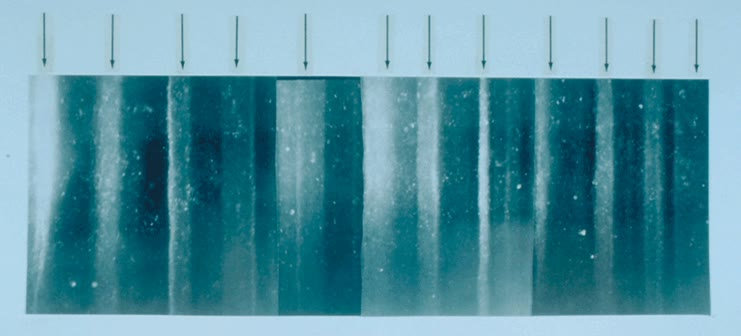
\includegraphics[width=0.72\linewidth]{images/book4/b2-24-gisp2-layers.jpg}
\par\smallskip{\small Een stuk van de GISP2-ijskern uit centraal Groenland, van \qty{1855}{m}
diepte, van onderen belicht, met afwisselende zomer- en winterlagen (de pijlen zijn die van de
oorspronkelijke dia). Tijdens de droge noordelijke zomer wordt stof uit Arctisch Canada en de kust van Groenland
door de wind op de ijskap gebracht.
(Anthony Gow, U.S.\ Army Corps of Engineers CRREL, NOAA Paleoclimatology slide set, publiek domein,
via Wikimedia Commons.)}
\end{omfigure}
% ledger: photo:b2-24-gisp2, noaa:gisp2-layers

\begin{inthelab}[Een ijskern zagen]
\begin{minipage}[t]{0.54\linewidth}\vspace{0pt}
In een nationale ijskernfaciliteit worden de kernen in kokers bewaard, één meter kern per koker, in een
archiefvriezer bij \qty{-36}{\celsius}; de onderzoekers werken in een onderzoeksruimte bij
\qty{-24}{\celsius}. Wanneer een nieuwe kern aankomt, wordt een verwerkingslijn gevormd: onderzoekers en
personeel meten, catalogiseren en zagen elk stuk, met doorgaans 30 tot \qty{35}{m} per dag, zodat een
kern van \qty{1000}{m} lang zes tot acht weken vraagt. Eén onderzoeker schaaft de kern glad met een
schaafmachine en meet zijn elektrische geleidbaarheid, een sleutel om de lagen te bepalen en te dateren; een ander
zaagt de stukken waarvan de ingesloten lucht op koolstofdioxide en methaan zal worden geanalyseerd; de monsters worden
daarna verzonden naar de laboratoria die ze meten. Bij EPICA Dome C was elk monster van het
$\delta$D-profiel \qty{55}{cm} ijs.
\end{minipage}\hfill
\begin{minipage}[t]{0.42\linewidth}\vspace{0pt}
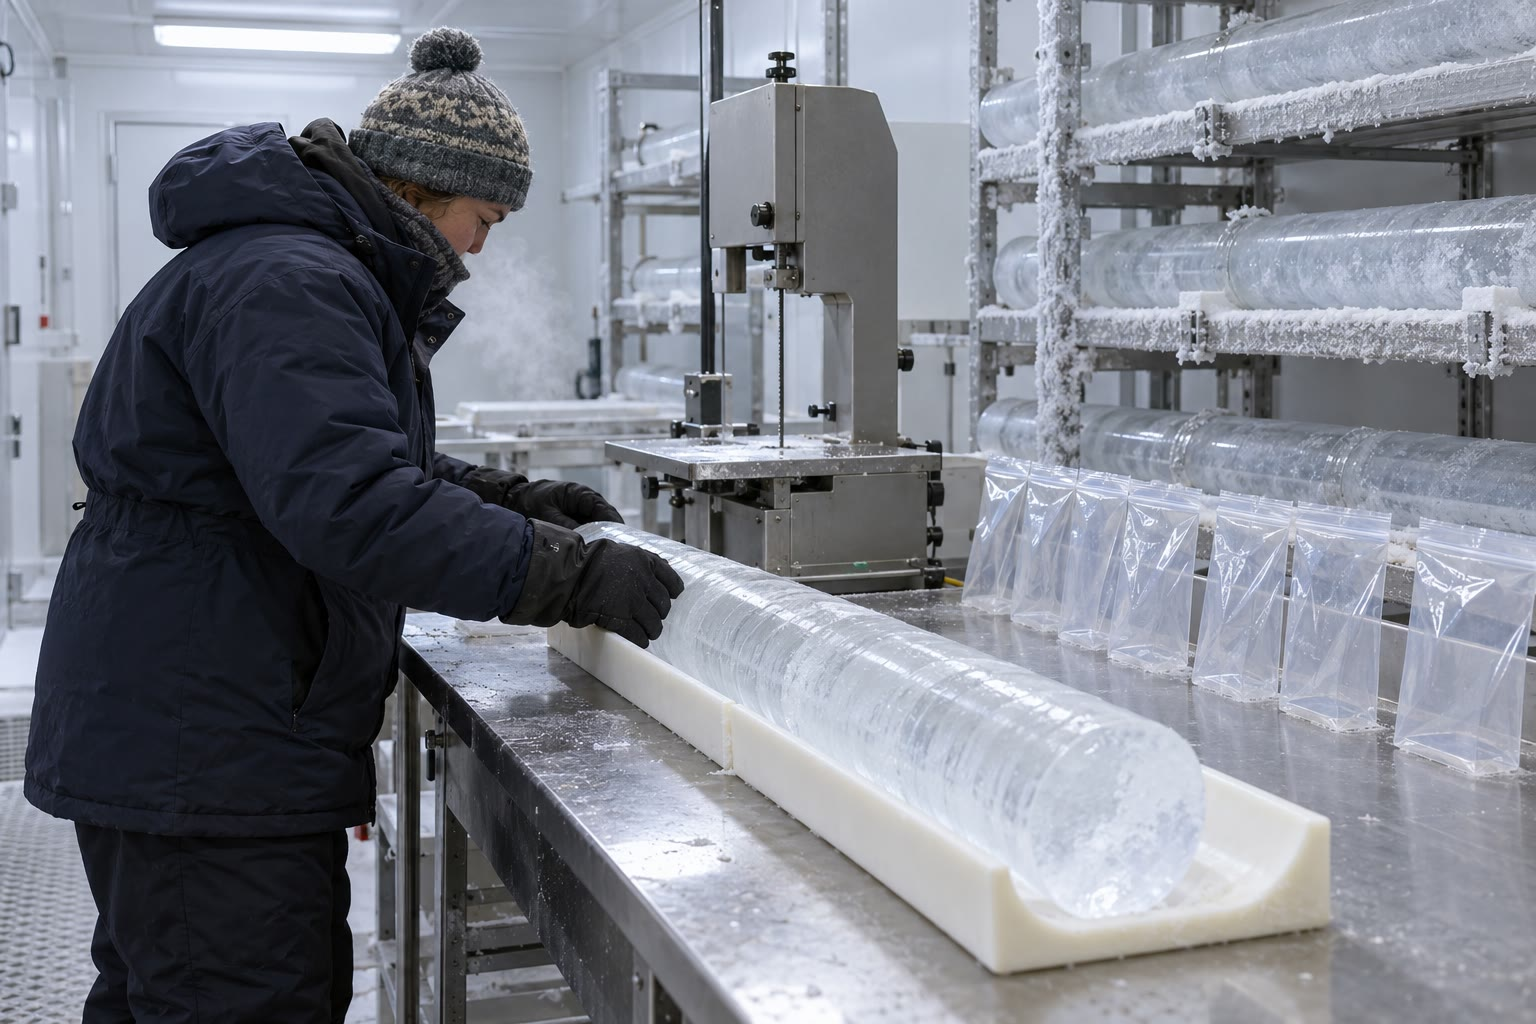
\includegraphics[width=\linewidth]{images/book4/ai/b2-24-cold-lab.jpg}

{\scriptsize Een stuk ijskern op de werkbank van een koudelaboratorium, naast een lintzaag en
monsterzakjes (door AI gegenereerde illustratie).}
\end{minipage}
\end{inthelab}
% ledger: nsficf:cpl, jouzel07:edc-corr

\section{Andere proxy's, andere archieven}\label{sec:b2:climate-proxies:others}

\subsection*{Het magnesium van schalen}

Het calciet van foraminiferen neemt een beetje magnesium op in plaats van calcium, en meer naarmate
het water warmer is. De verhouding hangt niet af van de isotopische samenstelling van het water, dus ze
geeft de temperatuur die de $\delta^{18}$O-vergelijking nodig heeft.

\begin{definition}[Mg/Ca-verhouding (proxy)]\label{def:b2:climate-proxies:mgca}
De \emph{Mg/Ca-verhouding (proxy)}\index{Mg/Ca-verhouding (proxy)} is de verhouding van magnesium tot calcium in
het calciet van foraminiferenschalen, in \unit{mmol/mol}, gebruikt als maat voor de temperatuur van
het water waarin de schaal groeide, via een exponentiële kalibratie
\[
  \text{Mg/Ca} = B\,\mathrm{e}^{A T},
\]
met $A$ dicht bij \qty{0.09}{\per\celsius} voor planktonische soorten en $B$ eigen aan de soort.
\end{definition}
% ledger: groeneveld19:anand, morley24:mgca, miller20:paleotemp

Met $A = 0.09$ groeit de verhouding met $\mathrm{e}^{0.09} - 1 = \qty{9.4}{\percent}$ per graad,
wat de temperatuur ook is. Voor één planktonische soort van koude wateren is de kalibratie die alleen uit de
temperatuur wordt voorspeld $\text{Mg/Ca} = 0.4\,\mathrm{e}^{0.09T}$; een aanpassing aan 235 schalen uit
planktonvangsten en de toppen van Noord-Atlantische kernen geeft $0.372\,\mathrm{e}^{0.0936T}$, met $r^2 = 0.90$.
Bij lage temperaturen wijken de gemeten verhoudingen af van de kromme, en die afwijking wordt toegeschreven aan
de concentratie van carbonaation in het zeewater: een proxy hangt zelden van slechts één variabele af.
Benthische soorten zijn minder gevoelig, ongeveer \qty{0.1}{mmol/mol} per graad voor magnesiumarme
soorten die in het sediment leven.
% ledger: morley24:mgca, wharton26:deep

\begin{omfigure}
\centering
% figdata/bachelor-2/proxies.py part calib
\begin{tikzpicture}
\begin{groupplot}[group style={group size=2 by 1, horizontal sep=1.7cm},
  tick label style={font=\scriptsize}, label style={font=\small}, height=5.2cm,
  width=0.48\linewidth]
\nextgroupplot[xmin=-2, xmax=14, ymin=0, ymax=3.8, xlabel={$T$ (\unit{\celsius})},
  ylabel={$\delta^{18}\mathrm{O}_{\mathrm{b}} - \delta^{18}\mathrm{O}_{\mathrm{sw}}$ (promille)},
  xtick={0,4,...,12}, title={a\enspace benthische $\delta^{18}$O}, title style={font=\scriptsize}]
\addplot[black, thick] table[x=T, y=dd_benthic] {figdata/out/bachelor-2-proxies-calib.dat};
\nextgroupplot[xmin=0, xmax=30, ymin=0, ymax=6.5, xlabel={$T$ (\unit{\celsius})},
  ylabel={Mg/Ca-verhouding (\unit{mmol/mol})}, xtick={0,5,...,30}, title={b\enspace planktonische Mg/Ca},
  title style={font=\scriptsize},
  legend style={font=\scriptsize, at={(0.03,0.97)}, anchor=north west, draw=none},
  legend cell align=left]
\addplot[ocRed, thick] table[x=T, y=mgca_pred] {figdata/out/bachelor-2-proxies-calib.dat};
\addlegendentry{$0.4\,\mathrm{e}^{0.09T}$}
\addplot[ocBlue, thick, densely dashed] table[x=T, y=mgca_fit]
  {figdata/out/bachelor-2-proxies-calib.dat};
\addlegendentry{$0.372\,\mathrm{e}^{0.0936T}$}
\end{groupplot}
\end{tikzpicture}
\par\smallskip{\small Twee kalibraties. (a) De benthische kalibratie van
\cref{prop:b2:climate-proxies:benthic}: het calciet is zwaarder dan het water (elk op zijn eigen
schaal), met \num{0.21} promille meer voor elke graad afkoeling. (b) De Mg/Ca van een planktonische
soort, zoals voorspeld uit de temperatuur alleen en zoals aangepast aan 235 schalen.}
\end{omfigure}
% ledger: miller20:paleotemp, morley24:mgca

Gemeten aan dezelfde schalen geven Mg/Ca en $\delta^{18}$O twee vergelijkingen voor twee onbekenden: Mg/Ca
geeft $T$, en \cref{prop:b2:climate-proxies:benthic} geeft dan
$\delta^{18}\mathrm{O}_{\mathrm{sw}}$, het ijsvolumesignaal. Toegepast op benthische schalen uit de diepe
noordwestelijke Atlantische Oceaan vindt de methode het water van het Laatste Glaciale Maximum slechts ongeveer
\qty{2}{\celsius} kouder dan nu ($-1.78 \pm \qty{0.56}{\celsius}$), terwijl schattingen uit
poriewater beide diepe watermassa's in de glaciale oceaan dicht bij het vriespunt plaatsen, $-1.1$ en
\qty{-1.9}{\celsius}, waar ze nu 2 tot \qty{4}{\celsius} en 0 tot \qty{1}{\celsius} warm zijn.
% ledger: miller20:paleotemp, wharton26:deep

\subsection*{Jaarringen}

\begin{definition}[Dendroklimatologie; kruisdatering]\label{def:b2:climate-proxies:dendro}
\emph{Dendroklimatologie}\index{dendroklimatologie} is de reconstructie van het vroegere klimaat uit de
jaarlijkse groeiringen van bomen: hun breedte, de dichtheid van hun hout en hun isotopische
samenstelling. \emph{Kruisdatering}\index{kruisdatering} is het afstemmen van het patroon van brede en
smalle ringen tussen bomen, dat aan elke ring zijn absolute kalenderjaar toekent en
ringen aan het licht brengt die in één boom plaatselijk ontbreken.
\end{definition}
% ledger: bebchuk26:crossdating, bebchuk26:absent-rings, ncei:tree-ring, ncei:proxy

Een ring is breder wanneer de omstandigheden de groei begunstigen. \omterm{def:b2:climate-proxies:dendro}{Kruisdatering} is betrouwbaar op klimatologisch extreme plaatsen, waar één
klimaatfactor de groei van alle bomen beperkt, zodat ze hetzelfde patroon delen; ze kan
mislukken waar geen enkele factor overheerst en waar veel ringen plaatselijk ontbreken.
Door de patronen van levende bomen, oud timmerhout en begraven hout te laten overlappen, wordt een chronologie
jaar voor jaar verder teruggetrokken; een recente studie dateerde een chronologie van 100 subfossiele taxusbomen uit Oost-Engeland op de
456 jaar van 2668 tot 2213 v.Chr., met de $\delta^{18}$O van meer dan \num{1500} van hun ringen
tegenover een absoluut gedateerde eikenchronologie. De International Tree-Ring Data Bank bevat de
ringbreedten, dichtheden, isotopen en chronologieën van meer dan \num{5000} locaties op zes continenten.
% ledger: ncei:proxy, bebchuk26:crossdating, bebchuk26:absent-rings, ncei:tree-ring

\subsection*{Grotten en meren}

\begin{definition}[Speleotheem; varve]\label{def:b2:climate-proxies:archives}
Een \emph{speleotheem}\index{speleotheem} is een minerale afzetting die in een grot uit grondwater
ontstaat: stalagmieten, stalactieten en andere vormen. Een \emph{varve}\index{varve} is
de afzetting van één jaar in het sediment van een meer- of zeebodem, meestal een paar laminae van contrasterende
samenstelling, de ene afgezet in de zomer en de andere in de rest van het jaar.
\end{definition}
% ledger: ncei:speleothem, mccarthy23:varves

\omterm{def:b2:climate-proxies:archives}{Speleothemen} groeien laag voor laag uit het grondwater dat een grot bereikt; de dikte van
hun lagen en hun isotopische registraties geven vroegere klimaatomstandigheden. Sommige hebben jaarbanden,
en sommige bevatten verbindingen die radiometrisch kunnen worden gedateerd. De tijdschaal van de Groenlandse kernen stemt tot op 800 jaar overeen met die van
de \omterm{def:b2:climate-proxies:archives}{speleothemen} van de Hulugrot, over de laatste \num{60000} jaar: twee
archieven, gedateerd met verschillende methoden, controleren elkaar.
% ledger: ncei:speleothem, svensson08:gicc05

\begin{omfigure}
\centering
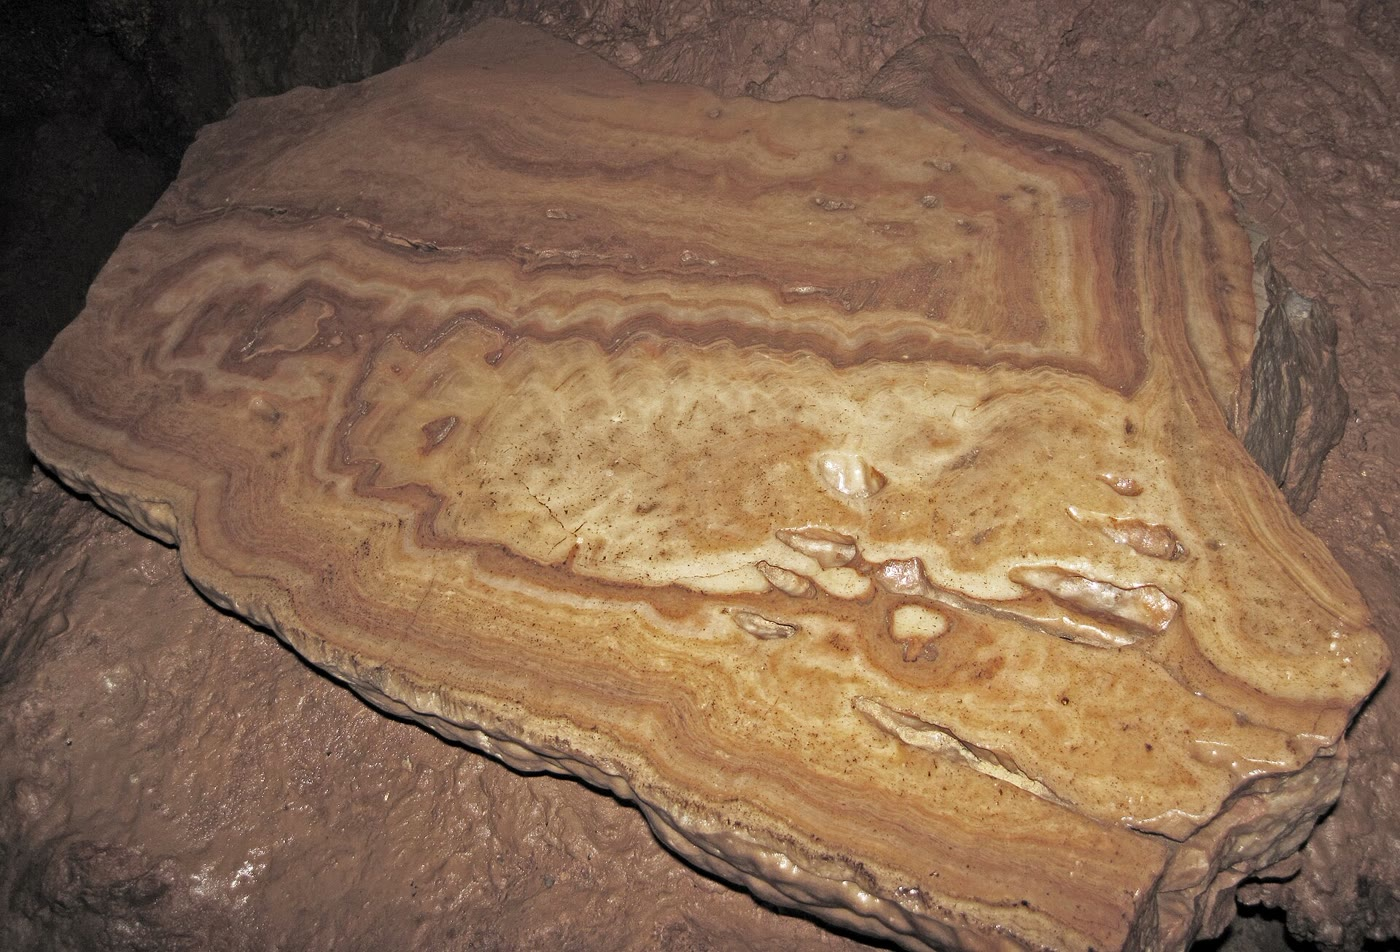
\includegraphics[width=0.62\linewidth]{images/book4/b2-24-speleothem.jpg}
\par\smallskip{\small Een gezaagde en gepolijste doorsnede van een \omterm{def:b2:climate-proxies:archives}{speleotheem} van calciet uit Diamond Caverns,
Kentucky, gekleurd door onzuiverheden van ijzeroxide: elke band was ooit het oppervlak van de afzetting.
(James St.~John, CC BY 2.0, via Wikimedia Commons.)}
\end{omfigure}
% ledger: photo:b2-24-speleothem

In het diepe bekken van Crawford Lake, in Ontario, bevat het bodemwater, zouter en alkalischer dan
het water erboven, geen dieren die groot genoeg zijn om het slib om te woelen, hoewel het goed
van zuurstof is voorzien, en elk jaar komt er een dubbellaag bij: een laag organisch materiaal, afgedekt door het
calciet dat elke zomer neerslaat uit het alkalische oppervlaktewater. Meersedimenten bewaren ook
het pollen van de omringende vegetatie, dat met pollenanalyse wordt gelezen; gevarveerd of niet, ze registreren
het land.
% ledger: mccarthy23:varves, mccarthy23:no-bioturbation, ncei:pollen

\section{Ouderdomsmodellen}\label{sec:b2:climate-proxies:age}

Een proxy zonder datum is een curiositeit. Elk archief heeft een betrekking nodig tussen diepte, ring of
band en ouderdom.

\begin{definition}[Ouderdomsmodel; tellen van jaarlagen]\label{def:b2:climate-proxies:age-model}
Een \emph{ouderdomsmodel}\index{ouderdomsmodel} is de functie die aan elke diepte van een archief een ouderdom toekent, met
haar onzekerheid. Het \emph{tellen van jaarlagen}\index{tellen van jaarlagen} bouwt een
ouderdomsmodel door van boven naar beneden de lagen te tellen die elk één jaar vastleggen (ijslagen, \omterm{def:b2:climate-proxies:archives}{varven},
banden), waarbij elke laag waarvan de jaarlijkse aard twijfelachtig is, wordt geteld als een half jaar plus of min
een half jaar.
\end{definition}
% ledger: svensson08:gicc05, mccarthy23:varves

\begin{method}[Een ouderdomsmodel opbouwen]\label{met:b2:climate-proxies:age-model}
\begin{enumerate}
  \item Waar het archief jaarlagen heeft: tel ze vanaf een bekende top en noteer de onzekere
        afzonderlijk.
  \item Waar het er geen heeft, of ze niet kunnen worden onderscheiden: leg \emph{ankerpunten} vast, dieptes die
        onafhankelijk zijn gedateerd, met radiokoolstof of andere radiometrische methoden, met een gedateerde vulkanische as, of door
        vergelijking met een goed gedateerde reeks.
  \item Interpoleer tussen de ankerpunten, lineair in de diepte als niets beters bekend is, of met een
        model van hoe het archief zich ophoopte en dunner werd.
  \item Draag de onzekerheid van elke stap over naar elke diepte.
\end{enumerate}
\end{method}
% ledger: svensson08:gicc05, noaa:gisp2-layers, ncei:speleothem

De Greenland Ice Core Chronology 2005, GICC05, telt jaarlagen in drie Groenlandse kernen, en
in het glaciale deel alleen in de NorthGRIP-kern, over de laatste \num{60000} jaar; haar ouderdommen worden
gegeven in jaren vóór 2000 n.Chr., geschreven b2k. De onzekere lagen, geteld als $\frac12 \pm \frac12$,
tellen op tot de \emph{maximale telfout}, die de auteurs als twee standaardafwijkingen beschouwen.
Aan het begin van het Holoceen, 11\,703 jaar b2k, bedraagt ze 50 jaar; aan het begin van het
Groenlandse interstadiaal 17, \num{59440} jaar b2k, bedraagt ze \num{1287} jaar.
% ledger: svensson08:gicc05, svensson08:table1

\begin{proposition}[Groei van een telfout]\label{prop:b2:climate-proxies:counting}
Laat een telling $n$ onzekere lagen bevatten, elk geteld als $\frac12$ met een fout met
standaardafwijking $\frac12$. Als de fouten van de lagen onafhankelijk zijn, is de standaardafwijking van het
totaal $\frac12\sqrt{n}$; als ze allemaal hetzelfde teken hebben, is de fout van het totaal
$\frac12 n$.
\end{proposition}

\begin{proof}
De variantie van een som van onafhankelijke fouten is de som van hun varianties: $n \times
(\frac12)^2$, met als vierkantswortel $\frac12\sqrt{n}$. Als elke laag zich in dezelfde richting vergist, tellen de
fouten op als getallen: $n \times \frac12$.
\end{proof}

Bij GI-17 betekenen de \num{1287} jaar maximale telfout \num{2574} onzekere lagen. Waren
hun fouten onafhankelijk, dan zou het totaal slechts $\frac12\sqrt{2574} = 25$ jaar onzeker zijn.
De lineaire som is de voorzichtige keuze: de twijfelachtige lagen van één stuk ijs worden beoordeeld door
dezelfde tellers met dezelfde criteria, en er is geen reden om te verwachten dat hun fouten elkaar opheffen.
Het oudere deel van de reeks werd onafhankelijk geteld door twee van de auteurs; hun tellingen
verschillen minder dan de absolute fout, al plaatselijk meer dan de uiteindelijke telfout. De
maximale telfout bedraagt gemiddeld ongeveer \qty{1}{\percent} van de tijd die een stuk beslaat in het Holoceen en
\qty{5}{\percent} in het glaciale deel.
% ledger: svensson08:gicc05, svensson08:table1, svensson08:two-counters

\begin{omfigure}
\centering
% figdata/bachelor-2/proxies.py part gicc05
\begin{tikzpicture}
\begin{groupplot}[group style={group size=2 by 1, horizontal sep=1.7cm},
  tick label style={font=\scriptsize}, label style={font=\small}, height=5.4cm,
  width=0.48\linewidth, xmin=0, xmax=62, xlabel={ouderdom GICC05 (\unit{ka} b2k)}]
\nextgroupplot[ymin=1450, ymax=2450, y dir=reverse, ylabel={diepte NorthGRIP (\unit{m})},
  title={a\enspace diepte en ouderdom}, title style={font=\scriptsize}]
\addplot[black, mark=*, mark size=1.1pt] table[x=age_ka, y=depth_m]
  {figdata/out/bachelor-2-proxies-gicc05.dat};
\nextgroupplot[ymode=log, ymin=2, ymax=30000, ylabel={onzekerheid (jaren)},
  title={b\enspace telonzekerheid}, title style={font=\scriptsize},
  legend style={font=\scriptsize, at={(0.03,0.97)}, anchor=north west, draw=none},
  legend cell align=left]
\addplot[ocRed, mark=*, mark size=1.1pt] table[x=age_ka, y=err_yr]
  {figdata/out/bachelor-2-proxies-gicc05.dat};
\addlegendentry{maximale telfout}
\addplot[ocBlue, mark=o, mark size=1.1pt] table[x=age_ka, y=err_random_yr]
  {figdata/out/bachelor-2-proxies-gicc05.dat};
\addlegendentry{indien onafhankelijk}
\end{groupplot}
\end{tikzpicture}
\par\smallskip{\small De GICC05-chronologie bij 18 klimaatgebeurtenissen van het begin van het Holoceen tot
\qty{59.44}{ka}: (a) diepte in de NorthGRIP-kern tegen ouderdom; de kromme vlakt af naarmate de
jaarlagen met de diepte dunner worden en elk duizendtal jaren minder meters ijs inneemt; (b) de maximale telfout, en de fout die hetzelfde aantal onzekere
lagen zou geven als hun fouten onafhankelijk waren (\cref{prop:b2:climate-proxies:counting});
logaritmische schaal. Gegevens: Svensson e.a.\ (2008), tabel 1.}
\end{omfigure}
% ledger: svensson08:table1, svensson08:gicc05

Jaarlagen worden met de diepte dunner, omdat het ijs vloeit en uitspreidt terwijl het zakt: tussen het begin van
het Holoceen en GI-1 is de gemiddelde laag \qty{3.75}{cm} dik in NorthGRIP; tussen GI-16 en
GI-17 \qty{1.54}{cm}; rond \qty{100}{ka} schatten stromingsmodellen haar op ongeveer \qty{1}{cm}. Hoe dunner de lagen, hoe moeilijker
ze uit elkaar te houden zijn.
% ledger: svensson08:table1, svensson08:gicc05

\section{Kalibratie}\label{sec:b2:climate-proxies:calibration}

Elk getal dat uit een proxy wordt afgelezen, komt via een kalibratie tot stand.

\begin{definition}[Proxykalibratie]\label{def:b2:climate-proxies:calibration}
Een \emph{proxykalibratie}\index{proxykalibratie} is de empirische of theoretische betrekking die
de waarde van een proxy omzet in de klimaatvariabele waarvoor ze staat, vastgesteld op monsters waarvan
beide bekend zijn, samen met haar onzekerheid en het bereik van omstandigheden waarbinnen ze
geldig is.
\end{definition}
% ledger: morley24:mgca, miller20:paleotemp

De monsters waarvan beide bekend zijn, zijn modern: schalen gevangen in planktonnetten, de toppen van sedimentkernen vergeleken met het water erboven, recente sneeuw vergeleken met de
temperatuur van haar locatie, de buitenste ringen van bomen vergeleken met de registraties van een weerstation.
De betrekking wordt dan met de kleinstekwadratenmethode aangepast; voor een exponentiële wet zoals de
Mg/Ca-kalibratie gebeurt de aanpassing op de logaritme, die $\text{Mg/Ca} = B\,\mathrm{e}^{AT}$ omzet in
de rechte $\ln(\text{Mg/Ca}) = \ln B + AT$. Een kalibratie wordt gevalideerd op monsters die
niet zijn gebruikt om haar aan te passen: een deel van de moderne gegevens wordt opzijgezet en voorspeld.
% ledger: morley24:mgca, werner18:slopes, ncei:tree-ring

Drie grenzen blijven. Een kalibratie die over de ruimte is gemeten, van plaats tot plaats vandaag, geldt misschien niet
in de tijd, zoals het Groenlandse ijs heeft laten zien. Een kalibratie die over het huidige bereik van omstandigheden is gemeten,
moet voorzichtig worden geëxtrapoleerd: de Mg/Ca van schalen wijkt bij lage temperaturen af van haar wet, waar
een andere variabele, het carbonaation, het overneemt. En een betrekking die over een klein bereik lineair is,
is dat misschien niet over een groot bereik, zoals het \omterm{def:b2:climate-proxies:ice-volume}{ijsvolume-effect} dat niet is. De methode van dit hoofdstuk
beantwoordt ze op dezelfde manier: meet twee onafhankelijke proxy's aan hetzelfde monster en laat elk
de andere controleren.
% ledger: werner18:slopes, morley24:mgca, rohling21:linear

\section*{Oefeningen}\label{sec:b2:climate-proxies:exercises}

Gegevens voor de oefeningen, tenzij anders vermeld: gemiddelde oceaandiepte $H = \qty{3682.2}{m}$,
oceaanoppervlak \qty{361.84e6}{km^2}; de benthische kalibratie van \cref{prop:b2:climate-proxies:benthic}; de
planktonische kalibratie $\text{Mg/Ca} = 0.4\,\mathrm{e}^{0.09T}$ (\unit{mmol/mol}, \unit{\celsius});
$\delta$-waarden van water en ijs in promille \omterm{def:b2:isotope-geochemistry:standards}{VSMOW}, van calciet in promille \omterm{def:b2:isotope-geochemistry:standards}{VPDB}.
% ledger: charette:ocean-volume, miller20:paleotemp, morley24:mgca

\begin{exercise}[$\star$]\label{exo:b2:climate-proxies:1}
Vandaag bevat het continentale ijs ongeveer \qty{27.5e6}{km^3} en de oceaan \qty{1350e6}{km^3}
water (beschouw de volumes als hoeveelheden water). (a) Als het ijs een gemiddelde $\delta^{18}$O van $-30$
promille heeft en de oceaan 0, wat is dan de $\delta^{18}$O van de hele hydrosfeer, het zoete
water verwaarloosd? (b) Als al het ijs smolt, wat zou de $\delta^{18}$O van de oceaan dan worden? (c) Welk
deel van het water is ijs?
\end{exercise}
% ledger: white13c9:ice-mass

\begin{exercise}[$\star$]\label{exo:b2:climate-proxies:2}
Een benthische schaal heeft $\delta^{18}\mathrm{O}_{\mathrm{b}} = 2.50$ promille. (a) Bereken haar
temperatuur als het zeewater $\delta^{18}\mathrm{O}_{\mathrm{sw}} = 0$ had. (b) Bereken ze als het
zeewater $+1.0$ promille had. (c) Een andere schaal, uit hetzelfde water bij $0$ promille, heeft
$2.71$ promille: hoeveel kouder was haar water?
\end{exercise}
% ledger: miller20:paleotemp

\begin{exercise}[$\star$]\label{exo:b2:climate-proxies:3}
(a) Bereken de Mg/Ca-verhouding van de planktonische kalibratie bij \qty{10}{\celsius} en bij
\qty{20}{\celsius}. (b) Met welke factor groeit de verhouding over deze tien graden, en met welk
percentage per graad? (c) Bereken de temperatuur van schalen met Mg/Ca = 2.0 en
\qty{1.0}{mmol/mol}.
\end{exercise}
% ledger: morley24:mgca

\begin{exercise}[$\star$]\label{exo:b2:climate-proxies:4}
Een chronologie van subfossiele taxusbomen loopt van 2668 tot 2213 v.Chr. (a) Hoeveel jaren beslaat ze,
beide eindjaren meegeteld? (b) Waarom verdient een chronologie die uit veel bomen is opgebouwd meer vertrouwen dan
de telling van de ringen van één boom? (c) Waarom zou \omterm{def:b2:climate-proxies:dendro}{kruisdatering} gemakkelijker zijn voor
bomen nabij de koude boomgrens dan voor bomen in een mild, vochtig laaglandbos?
\end{exercise}
% ledger: bebchuk26:crossdating

\begin{exercise}[$\star\star$]\label{exo:b2:climate-proxies:5}
(a) Bereken met \cref{prop:b2:climate-proxies:mass-balance} het \omterm{def:b2:climate-proxies:ice-volume}{ijsvolume-effect} voor een
zeespiegeldaling van \qty{125}{m} en van \qty{134}{m}, met ijs van $-40$ promille. (b) Bereken het voor
\qty{130}{m} met ijs van $-30$, $-35$ en $-50$ promille. (c) Welke gemiddelde samenstelling van het ijs
zou het effect van een daling van \qty{130}{m} gelijk maken aan de \num{1.0} promille gemeten in
poriewater? Vergelijk met de samenstellingen van de huidige ijskappen.
\end{exercise}
% ledger: ipcc:lgm-sea, white:d18o, miller20:ice-cal, wharton26:deep

\begin{exercise}[$\star\star$]\label{exo:b2:climate-proxies:6}
Vergelijk de twee kalibraties van de Mg/Ca van dezelfde planktonische soort: de kalibratie die alleen uit de
temperatuur wordt voorspeld, $0.4\,\mathrm{e}^{0.09T}$, en de aanpassing $0.372\,\mathrm{e}^{0.0936T}$. (a) Bij
welke temperatuur komen ze overeen? (b) Met welk percentage is bij \qty{2}{\celsius} de aangepaste verhouding
lager dan de voorspelde? (c) Een schaal die bij \qty{2}{\celsius} groeide, volgt de aangepaste wet; welke
temperatuur zou de voorspelde wet ervoor geven?
\end{exercise}
% ledger: morley24:mgca

\begin{exercise}[$\star\star$]\label{exo:b2:climate-proxies:7}
In de NorthGRIP-kern ligt het begin van het Holoceen op \qty{1492.45}{m} en \num{11703} jaar
b2k, het begin van GI-1 op \qty{1604.64}{m} en \num{14692} jaar; het begin van GI-16 op
\qty{2402.55}{m} en \num{58280} jaar, dat van GI-17 op \qty{2420.44}{m} en \num{59440} jaar.
(a) Bereken de gemiddelde dikte van de jaarlagen in elk interval. (b) Waarom zijn ze dieper
dunner? (c) Waarom wordt het \omterm{def:b2:climate-proxies:age-model}{tellen van jaarlagen} op een bepaalde diepte onmogelijk?
\end{exercise}
% ledger: svensson08:table1, svensson08:gicc05

\begin{exercise}[$\star\star$]\label{exo:b2:climate-proxies:8}
Gebruik de eerste twee ankerpunten van \cref{exo:b2:climate-proxies:7}, met maximale telfouten van 50
en 93 jaar. (a) Geef door lineaire interpolatie in de diepte de ouderdom van het ijs op \qty{1550}{m}.
(b) Druk die uit in jaren vóór 1950. (c) Interpoleer de onzekerheid op dezelfde manier.
\end{exercise}
% ledger: svensson08:table1

\begin{exercise}[$\star\star$]\label{exo:b2:climate-proxies:9}
De maximale telfout van GICC05 is 93 jaar bij GI-1 en \num{1287} jaar bij GI-17. (a) Hoeveel
onzekere lagen stelt elk voor? (b) Wat zou de onzekerheid zijn als de fouten van deze
lagen onafhankelijk waren, elk met een standaardafwijking van een half jaar? (c) Met welke factor overtreft de
lineaire som telkens de onafhankelijke schatting, en waarom groeit de factor met de diepte?
\end{exercise}
% ledger: svensson08:gicc05, svensson08:table1

\begin{exercise}[$\star\star\star$]\label{exo:b2:climate-proxies:10}
Bij EPICA Dome C is de gemiddelde $\delta$D van het ijs $-396.6$ promille over de laatste tweeduizend jaar
en $-441.7$ promille over 19 tot \qty{23}{ka}. (a) De Antarctische ruimtelijke helling van $\delta^{18}$O is
\num{0.8} promille per graad. Zet ze met de \omterm{prop:b2:isotope-geochemistry:mwl}{meteorische waterlijn} om in een helling van $\delta$D en
schat de glaciale afkoeling. (b) De glaciale oceaan was \num{1.0} promille zwaarder in
$\delta^{18}$O, dus de sneeuw die eruit ontstond, was ook zwaarder. Corrigeer de glaciale $\delta$D, aannemend dat de $\delta$D van de oceaan
acht keer zoveel veranderde, en schat de afkoeling opnieuw.
(c) De gepubliceerde anomalie is $-0.09$ en \qty{-9.39}{\celsius} voor de twee perioden; welke helling van
$\delta$D per graad impliceert dat, en welke andere correctie bevat de gepubliceerde reeks?
\end{exercise}
% ledger: data:b4-proxies, werner18:slopes, kc98:mwl, wharton26:deep, jouzel07:edc-corr

\begin{exercise}[$\star\star\star$]\label{exo:b2:climate-proxies:11}
Een kalibratie van de Mg/Ca van een planktonische soort gebruikt zes monsters van kerntoppen (watertemperatuur,
Mg/Ca uitgedrukt in \unit{mmol/mol}): (4, 0.59), (8, 0.80), (12, 1.21), (16, 1.65), (20, 2.47), (24, 3.41).
(a) Pas $\ln(\text{Mg/Ca}) = \ln B + AT$ aan met de kleinstekwadratenmethode, en geef $A$ en $B$. (b) Bereken de
residuen van de logaritme en vergelijk de aanpassing met de wet $0.4\,\mathrm{e}^{0.09T}$. (c) Geef de
temperatuur van een glaciale schaal met Mg/Ca = 1.30. (d) Een schaal heeft Mg/Ca = 0.45: bereken haar
temperatuur en zeg waarom deze waarde minder vertrouwen verdient dan de vorige.
\end{exercise}
% ledger: morley24:mgca

\begin{exercise}[$\star\star\star$]\label{exo:b2:climate-proxies:12}
Een ijskap groeit in twee stappen: eerst wordt \qty{60}{m} zeeniveau opgeslagen als ijs van $-30$ promille,
daarna nog \qty{70}{m} als ijs van $-45$ promille. (a) Toon aan dat de massabalans van
\cref{prop:b2:climate-proxies:mass-balance} voor meerdere ijsvoorraden $(H - h)\,\Delta\delta = -\sum_i h_i\delta_i$
wordt, en bereken het \omterm{def:b2:climate-proxies:ice-volume}{ijsvolume-effect} na elke stap. (b) Wat is de gemiddelde
samenstelling van het ijs aan het einde? (c) Een lineaire regel, gekalibreerd op de eindtoestand, zet
$\Delta\delta$ om in zeeniveau. Welke zeespiegeldaling zou hij voor de eerste stap afleiden, en waarom
vergist hij zich?
\end{exercise}
% ledger: rohling21:linear, white:d18o, miller20:ice-cal

\begin{problem}[{Weekendprobleem --- Eén schaal, twee signalen}]\label{pb:b2:climate-proxies:1}
Hoeveel kouder was de diepe oceaan tijdens het Laatste Glaciale Maximum? De $\delta^{18}$O van benthische schalen
vermengt het antwoord met het volume van het ijs; dit probleem scheidt de twee. Gebruik de gegevens van de
oefeningen; het zeeniveau stond 125 tot \qty{134}{m} lager dan nu, en het ijs van de Noord-Amerikaanse
ijskap had vermoedelijk een $\delta^{18}$O van ongeveer $-40$ promille.

\medskip\noindent\textbf{Deel I --- Het ijs op het land.}
\begin{enumerate}
  \item Bereken het volume water dat door een zeespiegeldaling van \qty{130}{m} aan de oceaan wordt onttrokken.
  \item Bereken het \omterm{def:b2:climate-proxies:ice-volume}{ijsvolume-effect} van die daling met ijs van $-40$ promille.
  \item Bereken het voor dalingen van \qty{125}{m} en \qty{134}{m}.
  \item Bereken het voor \qty{130}{m} met ijs van $-35$ en van $-50$ promille. Welke onzekerheid
        weegt zwaarder, die van het zeeniveau of die van het ijs?
  \item Het poriewater van glaciale sedimenten geeft $1.0 \pm 0.1$ promille. Welke gemiddelde samenstelling
        van het ijs zou een daling van \qty{130}{m} vergen om dat te geven?
  \item Bereken de verschuiving per meter zeeniveau voor kleine dalingen met ijs van $-40$ promille, en
        vergelijk met de waarde van \num{0.011} promille per meter, afgeleid uit gedateerde zeeniveaus.
\end{enumerate}

\medskip\noindent\textbf{Deel II --- Twee thermometers.}
\begin{enumerate}[resume]
  \item Toon met \cref{prop:b2:climate-proxies:benthic} aan dat een afkoeling van \qty{1}{\celsius} bij
        constante samenstelling van het water $\delta^{18}\mathrm{O}_{\mathrm{b}}$ met \num{0.21} promille verhoogt.
  \item Bereken $\delta^{18}\mathrm{O}_{\mathrm{b}}$ van een benthische schaal die vandaag groeit in water van
        \qty{2.0}{\celsius} met $\delta^{18}\mathrm{O}_{\mathrm{sw}} = 0$.
  \item Bereken ze voor een glaciale schaal die groeide in water van \qty{-1.0}{\celsius} met
        $\delta^{18}\mathrm{O}_{\mathrm{sw}} = +1.0$ promille. Wat is de verandering tussen de twee
        schalen, en welk deel ervan komt door de samenstelling van het water?
  \item Een planktonische schaal heeft Mg/Ca = \qty{2.0}{mmol/mol}. Bereken haar temperatuur.
  \item Magnesiumarme benthische schalen winnen ongeveer \qty{0.1}{mmol/mol} per graad. Een glaciale schaal heeft
        een Mg/Ca die \qty{0.18}{mmol/mol} lager is dan die van een moderne schaal van dezelfde soort van dezelfde
        plaats. Welke afkoeling wijst dat aan?
  \item Waarom geeft Mg/Ca een temperatuur die niet afhangt van het volume van het ijs?
\end{enumerate}

\medskip\noindent\textbf{Deel III --- Het restant.}
De stapelreeks LR04 geeft vandaag \num{3.23} promille en gemiddeld \num{4.92} promille over 19 tot
\qty{23}{ka}.
\begin{enumerate}[resume]
  \item Bereken de verandering van de stapelreeks tussen vandaag en het Laatste Glaciale Maximum.
  \item Als ze volledig \omterm{def:b2:climate-proxies:ice-volume}{ijsvolume-effect} was, met ijs van $-40$ promille, welke zeespiegeldaling zou ze dan
        impliceren (keer \cref{prop:b2:climate-proxies:mass-balance} om)? Is dat in overeenstemming met de
        aanwijzingen over het zeeniveau?
  \item Neem het \omterm{def:b2:climate-proxies:ice-volume}{ijsvolume-effect} van vraag 2. Welk restant blijft over voor de temperatuur, en
        welke afkoeling van het diepe water geeft het?
  \item Neem in plaats daarvan de poriewaterwaarde, \num{1.0} promille. Welk restant en welke afkoeling?
  \item Een andere reconstructie gebruikt \num{0.25} promille per graad. Herhaal de twee schattingen daarmee.
  \item Vandaag is het Noord-Atlantisch Diepwater 2 tot \qty{4}{\celsius} warm en het Antarctisch
        Bodemwater 0 tot \qty{1}{\celsius}; poriewater plaatst ze op $-1.1$ en \qty{-1.9}{\celsius}
        in de glaciale oceaan, en de Mg/Ca van benthische schalen vindt de diepe noordwestelijke Atlantische Oceaan
        slechts ongeveer \qty{1.8}{\celsius} kouder. Welk bereik van afkoeling geven deze, en welke van de
        twee schattingen van de vragen 15 en 16 ondersteunen ze?
\end{enumerate}

\medskip\noindent\textbf{Deel IV --- Het zicht vanuit het ijs.}
Bij EPICA Dome C is de gemiddelde $\delta$D $-396.6$ promille over de laatste tweeduizend jaar en
$-441.7$ promille over 19 tot \qty{23}{ka}; de gepubliceerde temperatuuranomalie is $-0.09$ en
\qty{-9.39}{\celsius}.
\begin{enumerate}[resume]
  \item Bereken de verandering van $\delta$D.
  \item Schat met een $\delta^{18}$O-helling van \num{0.8} promille per graad en de \omterm{prop:b2:isotope-geochemistry:mwl}{meteorische waterlijn}
        de afkoeling bij Dome C.
  \item Bereken de gepubliceerde afkoeling en de helling van $\delta$D per graad die ze impliceert.
  \item Het gemiddelde aardoppervlak was tijdens het Laatste Glaciale Maximum 5 tot \qty{7}{\celsius} kouder.
        Rangschik de afkoelingen van Dome C, van de aarde en van de diepe oceaan.
  \item Waarom kan de diepe oceaan niet zoveel zijn afgekoeld als het oppervlak van Antarctica?
  \item Samengevat: hoeveel kouder was de diepe oceaan, met de poriewatercorrectie voor het ijsvolume,
        tijdens het Laatste Glaciale Maximum dan nu?
\end{enumerate}
\end{problem}
% ledger: charette:ocean-volume, ipcc:lgm-sea, miller20:ice-cal, white:d18o, white13c9:ice-volume, wharton26:deep, miller20:paleotemp, morley24:mgca, data:b4-proxies, rohling21:linear, werner18:slopes, kc98:mwl, ipcc:lgm-cooling
